% Hill box: geometry and boundary conditions of the clamped gel slab.
% Build: pdflatex hill_box_bcs.tex && pdftocairo -svg hill_box_bcs.pdf hill_box_bcs.svg
\documentclass[tikz,border=4pt]{standalone}
\usetikzlibrary{arrows.meta,patterns,calc}
\tikzset{
	edge/.style={thick},
	hidden/.style={thin,dashed,gray},
	clamp/.style={pattern=north east lines,pattern color=red!60!black},
	drained/.style={fill=cyan!10},
	ax/.style={-{Latex[length=2mm]}},
}
\begin{document}
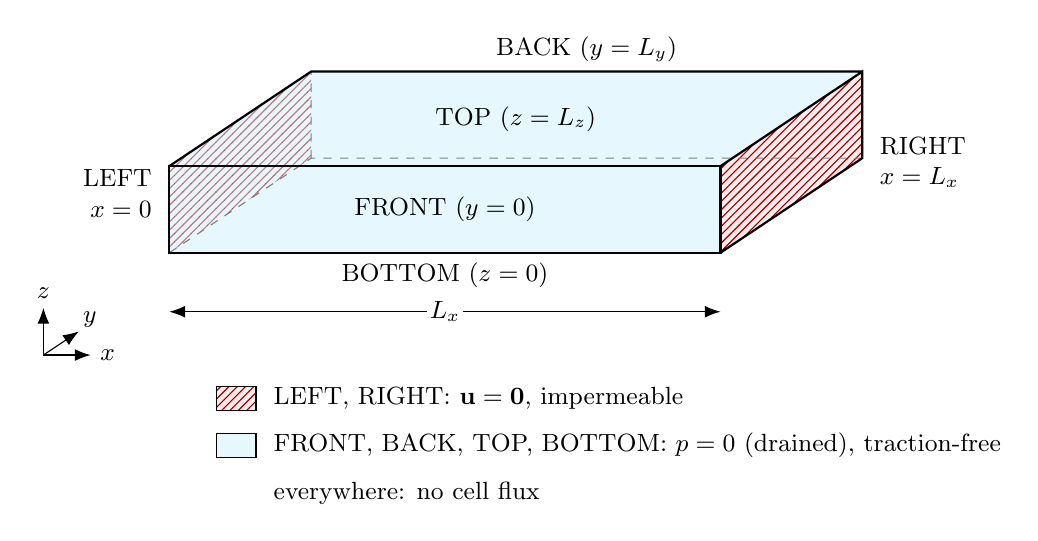
\begin{tikzpicture}[font=\small]
	% slab [0,Lx]x[0,Ly]x[0,Lz] in oblique projection (z exaggerated)
	\coordinate (O) at (0,0); \coordinate (X) at (7,0); \coordinate (Y) at (1.8,1.2); \coordinate (Z) at (0,1.1);
	\coordinate (XY) at ($(X)+(Y)$); \coordinate (XZ) at ($(X)+(Z)$); \coordinate (YZ) at ($(Y)+(Z)$);
	\coordinate (XYZ) at ($(X)+(Y)+(Z)$);
	% drained faces (FRONT, TOP)
	\fill[drained] (O) -- (X) -- (XZ) -- (Z) -- cycle;
	\fill[drained] (Z) -- (XZ) -- (XYZ) -- (YZ) -- cycle;
	% clamped faces (LEFT hidden, RIGHT visible)
	\fill[clamp,opacity=0.5] (O) -- (Y) -- (YZ) -- (Z) -- cycle;
	\fill[red!8] (X) -- (XY) -- (XYZ) -- (XZ) -- cycle;
	\fill[clamp] (X) -- (XY) -- (XYZ) -- (XZ) -- cycle;
	% edges
	\draw[hidden] (O) -- (Y) -- (XY) (Y) -- (YZ);
	\draw[edge] (O) -- (X) -- (XZ) -- (Z) -- cycle;
	\draw[edge] (X) -- (XY) -- (XYZ) -- (XZ) (Z) -- (YZ) -- (XYZ);
	% face labels
	\node at ($(O)!0.5!(XZ)$) {FRONT $(y = 0)$};
	\node at ($(Z)!0.5!(XYZ)$) {TOP $(z = L_z)$};
	\node[below] at ($(O)!0.5!(X)$) {BOTTOM $(z = 0)$};
	\node[above] at ($(YZ)!0.5!(XYZ)$) {BACK $(y = L_y)$};
	\node[left,align=right] at (-0.1,0.75) {LEFT\\ $x = 0$};
	\node[right,align=left] at (8.9,1.15) {RIGHT\\ $x = L_x$};
	% dimensions
	\draw[{Latex[length=2mm]}-{Latex[length=2mm]},thin] ($(O)+(0,-0.75)$) -- node[fill=white,inner sep=1pt] {$L_x$} ($(X)+(0,-0.75)$);
	% axes
	\begin{scope}[shift={(-1.6,-1.3)}]
		\draw[ax] (0,0) -- (0.6,0) node[right] {$x$};
		\draw[ax] (0,0) -- (0.45,0.3) node[above right=-2pt] {$y$};
		\draw[ax] (0,0) -- (0,0.6) node[above] {$z$};
	\end{scope}
	% legend
	\begin{scope}[shift={(0.6,-1.85)}]
		\fill[red!8] (0,-0.15) rectangle (0.5,0.15); \fill[clamp] (0,-0.15) rectangle (0.5,0.15);
		\draw (0,-0.15) rectangle (0.5,0.15);
		\node[right] at (0.6,0) {LEFT, RIGHT: $\mathbf u = \mathbf 0$, impermeable};
		\fill[drained] (0,-0.75) rectangle (0.5,-0.45); \draw (0,-0.75) rectangle (0.5,-0.45);
		\node[right] at (0.6,-0.6) {FRONT, BACK, TOP, BOTTOM: $p = 0$ (drained), traction-free};
		\node[right] at (0.6,-1.2) {everywhere: no cell flux};
	\end{scope}
\end{tikzpicture}
\end{document}
